\chapter{Tijd}

\begin{blockquotebox}
    Mensen ervaren de voortdurende stroom van tijd. Ze worden geboren, groeien op, verouderen en sterven uiteindelijk. Hun tijd is beperkt. Dit vereist dat ze economisch moeten handelen met deze tijd, vergelijkbaar met hoe ze omgaan met andere beperkte middelen. Het economisch handelen met tijd, ook bekend als economiseren, is opmerkelijk omdat de volgorde van tijd uniek en onherroepelijk is.\footnotemark
    \par\raggedleft--- Ludwig von Mises\index{Ludwig von Mises}
\end{blockquotebox}
\autocite{24}

\section{Het ultieme middel}

\lettrine{M}enselijke handelingen vinden plaats door tijd heen. Alle economische beslissingen vinden plaats op een moment in de tijd, en voor productie\index{productie} is tijd nodig. Omdat de mens sterfelijk is, is zijn tijd op de aarde beperkt, en deze beperking maakt het tot een economisch\index{economisch} goed en geeft het waarde. De onomkeerbare aard van de tijd maakt het een uniek economisch\index{economisch} goed. Je kunt de tijd die je aan iets besteedt niet terugkopen of je tijd oneindig blijven vergroten, zoals dat met andere goederen wel zou kunnen. Mises en de Oostenrijkse economen schreven welsprekend over het belang van het begrijpen van de tijdsdimensie van menselijk handelen\index{menselijk handelen} en de unieke aard van tijd als economisch\index{economisch} goed. Dit hoofdstuk zal ook voortbouwen op het werk van econoom Julian Simon\index{Julian Simon} om te beargumenteren dat menselijke tijd het ultieme middel is en dat economische schaarste\index{schaarste} een gevolg is van de schaarste\index{schaarste} van menselijke tijd. Het bezuinigen van tijd is de ultieme economiserende handeling, waaruit alle economische beslissingen voortvloeien. Als mensen meer tijd hebben, kunnen ze van elk economisch\index{economisch} goed meer maken.\autocite{25} Er zijn geen bindende fysieke beperkingen op de productie\index{productie} van economische goederen, en met de inzet van meer menselijke tijd en inspanning kan de productie\index{productie} van elk goed oneindig worden vergroot. De schaarste\index{schaarste} van tijd dwingt ons om keuzes te maken tussen verschillende economische goederen, wat de oorzaak is van hun schaarste.

Wanneer een kind in deze wereld wordt geboren, begint zijn tijd daarin. Die tijd is onzeker. Het kan maar een uur zijn, maar het kan ook een hele eeuw duren. Niemand weet hoelang hij of zij zal leven, maar iedereen beseft al snel dat het onmogelijk is om eeuwig te leven en dat zijn tijd alleen maar zal afnemen tot hij helemaal op is. Met dat besef, en gedurende het steeds volwassener worden, gaan mensen spaarzamer met tijd om.

In tegenstelling tot de relatieve en voortdurend afnemende schaarste\index{schaarste} van
materiële voorwerpen, neemt de absolute schaarste\index{schaarste} van de menselijke tijd
alleen maar toe. Dit is intuïtief waar voor individuen, aangezien groei
en veroudering de mens doet beseffen dat zijn tijd op de aarde alleen
maar beperkter wordt, waardoor het meer waarde krijgt. Het kan ook
gezien worden in de marktprijs die in de loop van de tijd voor
menselijke arbeid betaald wordt. Naarmate mensen meer tijd besteden aan
werken en productie\index{productie}, vergroten ze de overvloed aan materiële voorwerpen,
waardoor ze in de loop van de tijd in waarde dalen, gemeten in
menselijke arbeid. In zijn boek \textit{The
Ultimate Resource} stelt Simon dat menselijke tijd, of menselijke
arbeid, het ultieme productiemiddel is omdat het gebruikt kan worden om
alle economische goederen en productiemiddelen te maken.\autocite{26}
Het besteden van tijd aan een productieproces\index{productieproces} zou leiden tot een toename
in het aanbod van de productie\index{productie}, waardoor Simon stelt dat het gebruik van
de term ``resource'' (middel) om materiële goederen te beschrijven een
verkeerde benaming is, omdat materiële middelen de producten zijn van
het inzetten van het ultieme middel, dus menselijke tijd, om materialen
die praktisch oneindig overvloedig zijn om te zetten in bruikbare
economische goederen. De term ``middelen'' suggereert een vaste voorraad
die mensen aanspreken als ze consumeren, maar in werkelijkheid moeten
middelen eerst geproduceerd worden voordat ze geconsumeerd worden, en
hun productie\index{productie} wordt niet beperkt door hun fysieke overvloed op onze
enorme planeet, maar door de hoeveelheid tijd die mensen besteden aan de
productie\index{productie} ervan, en hun opportuniteitskosten gemeten in andere goederen.
Grondstoffen, metalen en brandstoffen worden ons niet als manna uit de
hemel gegeven; ze zijn het complexe resultaat van geavanceerde
productieprocessen om ze te produceren en in te zetten om aan menselijke
behoeften te voldoen.

Simons opvatting van menselijke tijd als het ultieme productiemiddel
verduidelijkt de aard van economische schaarste\index{schaarste}. Terwijl economen over
het algemeen de schaarste\index{schaarste} van materiële goederen als uitgangspunt namen
voor economische analyse, zou het nauwkeuriger zijn om schaarste\index{schaarste} te
begrijpen als een functie van de eindigheid van menselijke tijd. Hoewel
materiële goederen technisch gezien op aarde schaars zijn, liggen hun
absolute hoeveelheden binnen de planeet ver buiten ons vermogen om ze te
gebruiken. De hoeveelheid grondstoffen is daarom niet wat ze schaars
maakt. Wat ze voor ons schaars maakt, is de tijd die nodig is om ze te
produceren, aangezien die voor ons beperkt en begrensd is in een zeer
levendige betekenis.

\section{Opportuniteitskosten}

De schaarste\index{schaarste} van tijd is de reden waarom mensen niet alleen moeten
nadenken over de directe monetaire kosten van een activiteit, maar ook
over de \textbf{opportuniteitskosten} ervan: de
kosten van een activiteit bestaande uit de niet gerealiseerde waarde van
een andere activiteit die iemand had kunnen kiezen. Het feit dat onze
tijd schaars is, betekent dat we niet alles tegelijk kunnen doen. We
moeten kiezen. Zelfs als fysieke middelen geen beperking zouden zijn, is
de tijd die nodig is om activiteiten uit te voeren altijd een beperkende
factor, en mensen moeten elke keer als ze aan een activiteit deelnemen
rekening houden met de alternatieven die ze er voor opgeven.

De onvermijdelijkheid van de dood en de eindigheid van tijd, en dus de
schaarste\index{schaarste} ervan, maken een constante afweging van opportuniteitskosten
noodzakelijk, en daaruit komt al het economisch\index{economisch} denken en handelen van
de mens voort. Alle menselijke handelingen verbruiken tijd en gaan
daarom ten koste van niet gekozen handelingen. Als we schaarste\index{schaarste} in het
algemeen begrijpen als een gevolg van de schaarste\index{schaarste} van tijd, begrijpen
we ook de opportuniteitskosten en waarom de economische manier van
denken altijd de kosten van het niet gekozen alternatief moet omvatten.
Omdat menselijke tijd schaars is, is hij waardevol voor mensen. Er is
dus altijd een alternatief waardevol tijdsgebruik beschikbaar voor een
individu, waarmee rekening gehouden moet worden.

\section{Materiële overvloed}

De meest gebruikelijke maatstaf om de overvloed aan grondstoffen te
bespreken is de bewezen reserve, die verwijst naar de hoeveelheden van
een grondstof waarvan definitief bekend is dat ze op bepaalde locaties
voorkomen en die met de huidige technologie en prijzen gewonnen kunnen
worden.\autocite{27}

Volgens deze maatstaf is de voorraad voor elk bekende natuurlijke
hulpbron op de lange termijn toegenomen. Naarmate we meer van een
grondstof verbruiken, wordt deze ingezet voor meer doeleinden, en dat
creëert meer vraag ernaar, waardoor er meer naar gezocht wordt en de
reserves\index{reserves} dus toenemen. Simon illustreert hoe de bewezen reserves\index{reserves} tussen
1950 en 1990 zijn toegenomen voor een aantal belangrijke industriële
metalen. De wereldbevolking bedroeg in 1950 ongeveer 2,5 miljard mensen,
en was in 1990 gegroeid tot ongeveer 5,32 miljard
mensen.\autocite{28} Gemeten in dollars van 2011, werd het wereldwijde bbp in 1950
geschat op \$9.250 miljard, en in 1990 op \$47.040
miljard.\autocite{29} Dus in een periode van veertig jaar waarin de
menselijke bevolking met een factor 2,13 groeide en waarin de menselijke
productie\index{productie} vervijfvoudigde, groeiden de bewezen reserves\index{reserves} van de meeste
metalen met hogere snelheden dan de bevolkingsgroei, in plaats van
uitgeput te raken. De bewezen reserves\index{reserves} van lood groeiden met een factor
3, zink met 4,21; koper met 5,66; ijzererts met 8,27; olie\index{olie} met 13,1;
fosfaat met 14 en bauxiet met 16,6.\autocite{30}

Het is duidelijk dat de bewezen reserves\index{reserves} geen redelijke maatstaf zijn
voor de totale hoeveelheid grondstoffen op aarde, maar eerder een
maatstaf voor de hoeveelheid moeite die we doen om grondstoffen te
zoeken en te exploreren. Bewezen reserves\index{reserves} zijn een maatstaf voor de
hoeveelheid grondstoffen die we zoeken met de huidige technologieën
tegen de huidige prijzen. Naarmate we van deze middelen gebruikmaken en
onze levensstandaard stijgt, ontwikkelen we betere technieken om te
graven, en delven we in meer gebieden, waardoor deze bewezen reserves\index{reserves}
groeien. Bewezen reserves\index{reserves} zijn slechts het topje van de reusachtige,
deels verborgen ijsberg van de totale voorraad grondstoffen van de
aarde, die we nooit met enige nauwkeurigheid kunnen schatten. De aarde
is enorm groot en de exacte samenstelling ervan is zeer moeilijk vast te
stellen vanaf het oppervlak. De hele aarde opgraven om een sluitende
inventarisatie te maken is een zinloze en onmogelijk dure klus die
niemand ooit serieus zou kunnen overwegen.

Het helpt om een idee te krijgen van de omvang van de aarde om Simons
bewering te volgen. De oppervlakte van de aarde is 510,1 miljoen km², en
de totale oppervlakte die tussen 2000 en 2017 voor mijnbouw werd
gebruikt, werd geschat op 57.277 km², oftewel 0,011\% van de oppervlakte
van de planeet.\autocite{31} Als de
aarde de grootte van een voetbalveld had (105 m × 68 m, oftewel 7140 m²),
zou de oppervlakte van alle mijnen ter wereld 0,785 m² zijn, ongeveer de
grootte van een klein bureau (een bureau van 122 cm × 61 cm heeft een
oppervlakte van 0,744 m²).

\begin{figure}[!htb]
\centering
    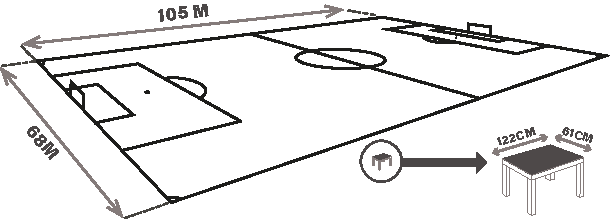
\includegraphics[width=\textwidth]{figures/fig2.pdf}
\caption[Als de aarde een voetbalveld was, zouden alle mijnen
een klein bureau zijn]{Als de aarde een voetbalveld was, zouden alle mijnen
een klein bureau zijn}
\label{fig2}
\end{figure}

De diameter van de aarde bedraagt 12.742 kilometer, terwijl de diepste mijn ter wereld, de Mponeng goudmijn nabij Johannesburg, slechts tussen 3,16 km en 3,84 km diep is, wat neerkomt op slechts 0,024\% tot 0,03\% van de aarddiameter. Ter illustratie: als de aarde een bal zou zijn met een diameter van 1 meter, dan zou het diepste gat dat we ooit in de aardkorst hebben geboord slechts 0,027 cm diep zijn, minder dan de dikte van drie boekpagina’s. Het merendeel van het aardoppervlak is onberoerd gebleven in de zoektocht naar grondstoffen, en op de paar plekken waar we wel hebben gegraven, hebben we letterlijk nauwelijks meer dan een krasje gemaakt. De grondstoffen die de mensheid in duizenden jaren heeft verbruikt en geëxploiteerd, vormen slechts een fractie van de overvloed die beschikbaar is binnen de verwaarloosbare 0,027\% van de aarddiameter.

De meeste mijnen zijn rond de 300 meter diep. Laten we bij het volgende
punt uitgaan van een zeer royale gemiddelde diepte van een mijn van 1
km. Dit zou betekenen dat het totale volume aan mijnen in de periode
tussen 2000 en 2017 zo'n 57.277 km\textsuperscript{3} was. Het volume van de aarde is
1.083.206.916.845,80 km³ (ongeveer een triljoen kubieke kilometer). Het
volume van alle mijnen op aarde is dus 0,00000529\% van het volume van
de aarde. Met andere woorden, de aarde is 18.911.725,8 keer zo groot als
alle mijnen die erop liggen en waaruit we al onze grondstoffen hebben
gehaald. Ter vergelijking, als het volume van de aarde dat van een
olympisch zwembad was, dan zouden alle mijnen ter wereld ruwweg de
grootte van een half glas hebben.\autocite{32}

\begin{figure}[!htb]
\centering
    \includegraphics[width=\textwidth]{figures/fig3.pdf}
\caption[Als de aarde een olympisch zwembad was, zouden al
onze mijnen een half glas zijn]{Als de aarde een olympisch zwembad was, zouden al
onze mijnen een half glas zijn}
\label{fig3}
\end{figure}

Als alle grondstoffen die mensen verbruiken afkomstig zijn uit het
equivalent van een half glas van het olympische zwembad dat de aarde is,
dan wordt het duidelijk waarom het zorgen maken over de totale
hoeveelheid grondstoffen zo misplaatst is. Als acht miljard mensen
kunnen leven van het equivalent van een half glas uit een olympisch
zwembad, dan is het duidelijk dat de totale hoeveelheid water in het
zwembad irrelevant is voor het menselijk leven en alle economische
overwegingen. De wereldbevolking zou moeten verdubbelen om uit een
olympisch zwembad de waarde van één glas te moeten produceren. Zelfs met
een enorme groei van de wereldbevolking zullen we nauwelijks een krasje
op het oppervlak van onze enorme, overvloedige planeet maken. Zelfs de
meest conservatieve schattingen komen tot de conclusie dat de totale
overvloed in de aardkorst van een bepaalde natuurlijk voorkomende
grondstof vele ontelbare veelvouden is van de totale hoeveelheid die
mensen ervan consumeren en die hoeveelheid vormt geen relevante limiet
of bindende beperking voor ons consumptieniveau. Het is heel
waarschijnlijk dat de totale overvloed in de aardkorst van een bepaald
metaal gelijk is aan miljoenen jaren menselijke consumptie\index{consumptie}. Zelfs als de
huidige, verondersteld niet-duurzame, consumptietrends duizenden jaren
zouden aanhouden, zouden we niet in staat zijn om de volledige inhoud
van de aarde aan een bepaald metaal op te maken. De hoeveelheid van elk metaal die we in een bepaald jaar kunnen produceren, wordt beperkt door de tijd en middelen die we eraan besteden en door de hoeveelheid andere goederen en diensten die we bereid zijn op te offeren voor de productie\index{productie} ervan.

Afgezien van het feit dat ze als illustratie in dit economieboek worden
gebruikt, zijn deze geaggregeerde metingen van de grondstoffen op aarde
volledig zinloze en irrelevante meetgegevens die geen rol spelen in de
economische beslissingen die waar dan ook door wie dan ook worden
genomen. Er zijn geen economische beslissingen die betrekking hebben op
de totale voorraad metaal op de aarde, en alle individuele economische
beslissingen met betrekking tot een middel worden marginaal gemaakt,
gebaseerd op de volgende marginale eenheid land die geëxploiteerd moet
worden, de marginale kosten van het winnen van de volgende eenheid, en
de marginale opbrengst die verwacht wordt van de verkoop ervan. Op geen
enkel moment kan een individu of entiteit een economische beslissing
nemen die betrekking heeft op de totale geaggregeerde voorraad van een
materiaal op aarde. Economische berekeningen worden voortdurend in de
marge gemaakt en hebben alleen betrekking op schaarse grondstoffen die
opportuniteitskosten met zich meebrengen. Mineralen in de aardkorst zijn
niet schaars en bieden geen nut voor mensen. Om er daarentegen bruikbare
materialen van te maken, moeten er echte beslissingen genomen worden
over de toewijzing van marginale eenheden van schaarse grondstoffen aan
de exploratie-, opgravings-, extractie-, raffinage- en
productieprocessen.

Een nuttige analogie hierbij is om de grondstoffen van de aarde te zien
als stenen, en onze consumptie\index{consumptie} van grondstoffen als het gebruik van
stenen om huizen te bouwen. Geen enkele economische beslissing hoeft
rekening te houden met de totale hoeveelheid stenen op aarde;
economische beslissingen hebben alleen betrekking op de toepassing van
schaarse middelen, arbeid, kapitaal\index{kapitaal} en land, op het proces van het
delven en toepassen van stenen. Het zou krankzinnig zijn voor een
huizenbouwer om zich bezig te houden met de beschikbaarheid van stenen
in de natuur, als al onze huizen een oneindig klein deel van de stenen
op aarde nodig hebben voor de bouw ervan. Voor de huizenbouwer is de enige economisch\index{economisch} urgente kwestie of hij toegang heeft tot de menselijke arbeid en het door mensen geproduceerde kapitaal\index{kapitaal} dat nodig is om die stenen in huizen te transformeren.

Waar we echt waarde aan hechten zijn niet de grondstoffen, maar
economische goederen die van grondstoffen gemaakt zijn. Daar is tijd
voor nodig, en dat is wat schaars is. Dat is de schaarste\index{schaarste} waaruit alle
andere schaarste\index{schaarste} voortkomt. De ruwe materie bestaat overal om ons heen,
maar de tijd om er economische goederen van te maken is schaars. Mensen
zijn geen passieve ontvangers van manna dat op kan raken. Mensen zijn de
producenten van al deze middelen, en wanneer de vraag naar deze
materialen toeneemt, is het handelen van de mensen die ze produceren en de
prikkels waarmee ze te maken krijgen, de belangrijkste bepalende factor
voor hun schaarste\index{schaarste}. Naarmate de vraag naar een natuurlijke hulpbron
toeneemt, worden ze gestimuleerd om er meer van te produceren en meer in
de productie\index{productie} ervan te investeren. Naarmate de productiviteit toeneemt,
zijn we in staat om grotere hoeveelheden van het aanbod van het goed te
verkrijgen per hoeveelheid tijd die in de productie\index{productie} ervan wordt
geïnvesteerd, wat betekent dat de reële prijs\index{prijs} van het goed, gemeten in
menselijke arbeid, zal blijven dalen. Dit feit wordt bevestigd door
tientallen jaren van gegevens over de grondstoffenmarkt.

Hoewel grondstofprijzen kunnen stijgen in nationale valuta en dat
meestal ook doen, is dat het gevolg van de devaluatie van nationale
valuta. Gemeten aan de loonkosten, of de prijs\index{prijs} van menselijke tijd,
dalen de prijzen van alle grondstoffen op de lange termijn, zelfs als de
consumptie\index{consumptie} gestaag toeneemt. In een wereld met hard geld\index{hard geld}, zoals onder de
goudstandaard\index{goudstandaard}, zou het volkomen normaal zijn om te verwachten dat de
prijzen van alle grondstoffen in de loop van de tijd consequent dalen,
met slechts af en toe een tijdelijke stijging door scherpe, plotselinge stijgingen van de vraag en de verstoringen van de productie\index{productie}. Goud, of wat
er ook als geld wordt gebruikt, zou altijd het goed zijn waarvan het
aanbod het langzaamst toeneemt, waardoor de eigenaars ervan er voor
altijd meer van alle andere goederen kunnen krijgen, waarvan het aanbod
sneller toeneemt.

Economen Gale Pooley en Marian Tupy hebben ter ere van Julian Simon\index{Julian Simon} een
economische index gemaakt die de prijzen van 50 basisproducten meet in
``loon''. Zij ontdekten dat de tijd die nodig is om een mandje van 50
basisproducten te verdienen in de periode tussen 1980 en 2020 met 75,2\%
is gedaald, wat betekent dat een uur werk in 2020 4,03 keer zoveel van
de 50 basisproducten kan kopen als in 1980, wat een jaarlijkse groei van
3,55\% en een verdubbeling van de overvloed aan basisproducten elke 20
jaar betekent.\autocite{33} Hoewel de menselijke bevolking in deze
40 jaar met 75,8\% is toegenomen, decennia die de grootste
bevolkingsgroei en de hoogste consumptie\index{consumptie} en levensstandaard in de
geschiedenis kenden, zijn de prijzen van 50 basisproducten met driekwart
gedaald, gemeten in arbeidstijd die nodig is om ze te kopen. Deze
gegevens kunnen alleen begrepen worden in de context van een oneindig
grote aarde waarvan de fysieke grenzen niet in de buurt van onze greep
liggen, een greep die beperkt wordt door de schaarste\index{schaarste} van onze tijd en
de opportuniteitskosten die gepaard gaan met het verhogen van de
productie\index{productie} van een bepaalde natuurlijke hulpbron.

\begin{figure}[!htb]
\centering
    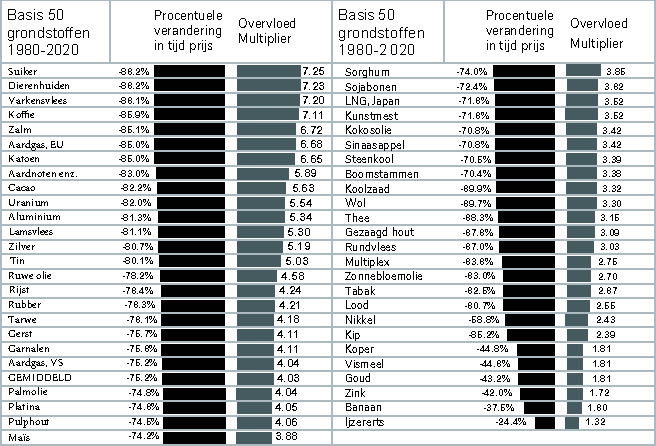
\includegraphics[width=\textwidth]{figures/fig4.pdf}
\caption[Veranderingen van prijzen gemeten in tijd en
overvloed van 50 basisproducten (1980 tot 2020)]{Veranderingen van prijzen gemeten in tijd en overvloed van 50 basisproducten (1980 tot 2020)}
\label{fig4}
\end{figure}

De enige schaarste\index{schaarste}, zoals Julian Simon\index{Julian Simon} op een briljante manier heeft
aangetoond, is de tijd die mensen hebben om deze goederen te produceren,
en daarom blijven de lonen wereldwijd stijgen, waardoor producten en
materialen voortdurend goedkoper worden als we ze meten in menselijke
arbeid. De enige `grondstof' waarvan de prijs\index{prijs} in de loop van de
geschiedenis bijna voortdurend is gestegen, is menselijke tijd, zoals we
zien als we naar lonen kijken. Naarmate we meer inventieve manieren
blijven vinden om de productie\index{productie} van fysieke hulpmiddelen te verhogen,
blijft hun reële prijs\index{prijs}, in menselijke tijd dalen, terwijl de waarde van
menselijke tijd blijft stijgen. Alleen met dit raamwerk kan men
begrijpen waarom de mensheid nog nooit zonder grondstoffen is komen te
zitten, zelfs niet na vele millennia van exploitatie van de aarde en de
niet aflatende voorspellingen van naderend onheil door uitputting van
natuurlijke hulpbronnen. Niet alleen is geen enkele grondstof uitgeput
geraakt, maar in feite blijven de reële prijzen dalen, blijft de
jaarlijkse productie\index{productie} van vrijwel alle grondstoffen elk jaar stijgen, en
zijn de bewezen reserves\index{reserves} van elke grondstof in de loop van de tijd
alleen maar toegenomen terwijl onze consumptie\index{consumptie} is gestegen, zoals
hierboven in de gegevens van Simon wordt vermeld. Als grondstoffen als
eindig moeten worden beschouwd, dan zouden de bestaande voorraden in de
loop van de tijd afnemen naarmate we meer consumeren. Maar zelfs als we
altijd meer verbruiken, blijven de prijzen dalen, en de technologische
verbeteringen voor het vinden en opgraven van grondstoffen stellen ons
in staat om meer ongebruikte voorraden te vinden.

Olie, het onmisbare smeermiddel van moderne economieën, is het beste
voorbeeld omdat er vrij betrouwbare statistieken voor zijn. Zoals Figuur
5 laat zien, blijven het olieverbruik en de olieproductie van jaar tot
jaar stijgen, terwijl de bewezen reserves\index{reserves} nog sneller toenemen. Volgens
gegevens van BP's Statistical Review of World Energy lag de jaarlijkse
olieproductie in 2015 46\% hoger dan in 1980, terwijl het verbruik 55\%
hoger lag. De oliereserves daarentegen zijn met 148\% toegenomen,
ongeveer het drievoudige van de toename in productie\index{productie} en verbruik.

\begin{figure}[!htb]
\centering
    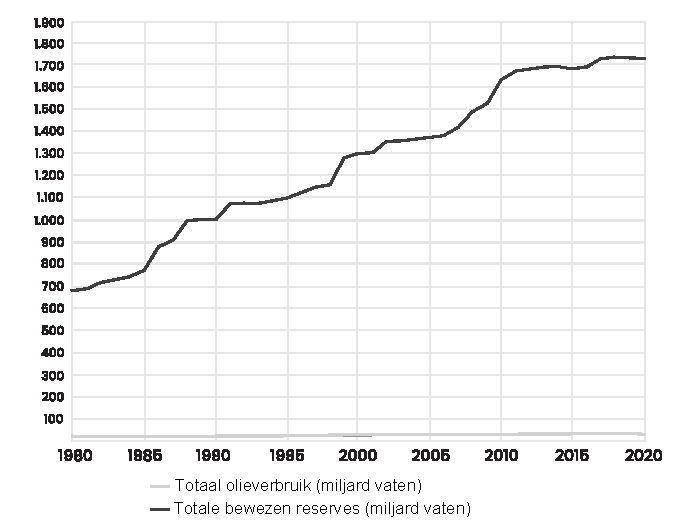
\includegraphics[width=\textwidth]{figures/fig5.pdf}
\caption[Olieverbruik en bewezen reserves\index{reserves}]{Olieverbruik en bewezen reserves\index{reserves}\footnotemark}
\label{fig5}
\end{figure}
\autocite{34}

Vergelijkbare statistieken kunnen worden opgesteld voor grondstoffen die
in verschillende hoeveelheden voorkomen in de aardkorst. De zeldzaamheid
van een grondstof bepaalt de relatieve kosten om deze uit de aarde te
halen. Meer voorkomende metalen, zoals ijzer en koper, zijn gemakkelijk
te vinden en daardoor relatief goedkoop. Zeldzamere metalen, zoals
zilver\index{zilver} en goud\index{goud}, zijn duurder. De limiet op hoeveel we van elk van deze
metalen kunnen produceren blijft echter de opportuniteitskosten van hun
productie\index{productie} vergeleken met elkaar, in subjectieve menselijke waardering,
en niet hun absolute hoeveelheid. Er is hiervoor geen beter bewijs dan
het feit dat goud\index{goud}, één van de (al dan niet) zeldzaamste metalen in de
aardkorst, al duizenden jaren wordt gedolven en nog steeds in steeds
grotere hoeveelheden wordt gedolven naarmate de technologie
voortschrijdt.

\begin{figure}[!htb]
\centering
    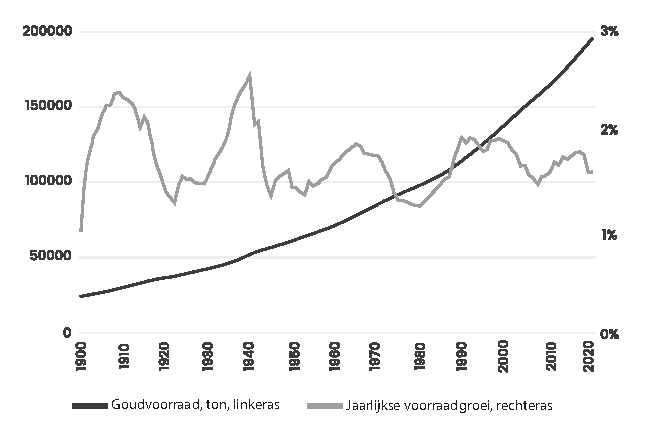
\includegraphics[width=\textwidth]{figures/fig6.pdf}
\caption[Wereldwijde jaarlijkse goudproductie]{Wereldwijde jaarlijkse goudproductie\footnotemark}
\label{fig6}
\end{figure}
\autocite{35}

Als er andere metalen zijn die zeldzamer zijn dan goud\index{goud}, dan zijn die
allemaal recent ontdekt en hebben we niet zoveel tijd besteed aan het
vinden van hun reserves\index{reserves} en het aanleggen van hun voorraden als bij goud\index{goud}.
Maar naar goud\index{goud} wordt al duizenden jaren gezocht en het wordt al duizenden jaren gedolven, en de
jaarlijkse productie\index{productie} ervan stijgt elk jaar, dus het heeft geen zin om in
praktische zin te spreken van een natuurlijk element dat beperkt is in
zijn hoeveelheid. Schaarste is alleen relatief ten opzichte van
materiële hulpmiddelen, waarbij de verschillen in de delvingskosten de
schaarste\index{schaarste} bepalen.


\section{Simons weddenschap}

Nadat de Amerikaanse president Richard Nixon in 1971 de inwisselbaarheid
van de Amerikaanse dollar\index{Amerikaanse dollar} in goud\index{goud} opschortte, begonnen alle prijzen
onverbiddelijk te stijgen, een trend die tot op de dag van vandaag
aanhoudt. Voor mensen die in de jaren `70 gewend waren aan relatief
stabiele prijzen onder de goudstandaard\index{goudstandaard}, leken deze prijsstijgingen een
teken van een economische apocalyps, omdat ze de indruk wekten dat al
onze kostbare grondstoffen uitgeput raakten. Terwijl de wereld werd
meegesleurd in de hysterie over de uitputting van grondstoffen en
overbevolking, was Simon niet tevreden met alleen maar schrijven om de
hysterie tegen te gaan. Hij probeerde de leegheid van de hysterici bloot
te leggen door Paul Ehrlich, een van de meest vooraanstaande hysterici
van de twintigste eeuw, uit te dagen voor een publieke weddenschap over
de kwestie.

Ehrlich had een groot aantal hysterische tirades gepubliceerd die het
niet waard zijn om in de bibliografie van dit boek opgenomen te worden,
waaronder de voorspelling dat verschillende essentiële hulpbronnen voor
de mensheid uitgeput zouden raken als gevolg van overbevolking, en
voegde daar typisch misantropische tirades over eugenetica en gedwongen
sterilisatie en andere maatregelen om de menselijke bevolking te
verminderen aan toe. Simon daagde Ehrlich uit om grondstoffen te noemen
waarvan hij zeker wist dat ze op zouden raken of veel schaarser zouden
worden over een periode langer dan een jaar, en Simon zou met hem om
\$1.000 wedden dat elk van deze grondstoffen aan het einde van de
periode reëel gezien daadwerkelijk goedkoper zou zijn.

De weddenschap moet voor Ehrlich als een zekere overwinning hebben geleken, zo vast stond hij achter zijn voorspellingen over de aanstaande schaarste van kritieke grondstoffen. Ehrlich koos 5 metalen uit en stelde een periode van 10 jaar, van 1980 tot 1990, vast om de prijsontwikkeling te volgen. Aan het eind van deze periode waren al deze metalen, in reële termen, goedkoper dan aan het begin. Dertig jaar later zijn de prijzen van deze metalen nog verder gedaald, terwijl hun jaarlijkse productie voortdurend toeneemt.

De reden dat de prijs\index{prijs} van al deze metalen daalde, is dat hun schaarste\index{schaarste}
relatief is, niet absoluut. Ze zijn schaars voor ons omdat de tijd en
middelen die nodig zijn om ze te produceren, moeten worden onttrokken
aan de productie\index{productie} van andere grondstoffen. Simon begreep dat naarmate de
menselijke bevolking toenam en de vraag naar deze metalen steeg, er meer
middelen aan de productie\index{productie} van deze metalen besteed zou worden, de
hoeveelheden zouden toenemen en de prijzen zouden dalen. De stijging van
de vraag zorgt voor een stijging van de prijzen, waardoor de producenten
van deze metalen meer winst maken, meer geld hebben om te investeren en
meer investeringen kunnen aantrekken. Deze investeringen gaan naar het
opsporen, winnen, raffineren en distribueren van de metalen, wat
allemaal leidt tot een stijging van de productiviteit, de productie\index{productie} per
eenheid input. Zoals meer in detail besproken zal worden in Hoofdstuk 4,
maken grotere kapitaalinvesteringen het mogelijk om complexere en
langere productiemethoden te gebruiken die een hogere productiviteit per
werknemer opleveren.

Als geoloog baseerde Ehrlich zijn visie op schaarste\index{schaarste} op de verhouding tussen de consumptie\index{consumptie} en de reserves\index{reserves} van metalen, zonder de invloed van menselijk handelen\index{menselijk handelen} op deze balans mee te wegen. In feite mat Ehrlich de bewezen reserves af tegen de jaarlijkse consumptie en berekende hoe lang de mensheid met deze reserves zou doen. Simon, als econoom, begreep de dynamiek achter de productie van deze metalen, zelfs zonder diepgaande kennis van de geologie. Door economie te zien als de studie van menselijk handelen, zoals besproken in het eerste hoofdstuk, erkende Simon dat de schaarste van metalen uiteindelijk afhing van de tijd die mensen bereid waren erin te investeren. Dit was op zijn beurt weer afhankelijk van de stimulans om deze grondstoffen te winnen, en niet zozeer van geologische beperkingen. Wanneer de vraag naar een metaal stijgt, is er niet slechts een beperkte hoeveelheid die op kan raken. Er zijn altijd nieuwe gebieden om te ontginnen en diepere mijnen om te graven.

\section{Tijdsvoorkeur}

Vanwege de eindigheid en onzekerheid van menselijke tijd kan niemand met zekerheid weten hoe lang hij zal leven of wanneer hij zal overlijden. Dit creëert
in de mens een \textbf{tijdsvoorkeur\index{tijdsvoorkeur}}, een universele voorkeur voor
vroegere boven latere voldoening van behoeften. Mensen consumeren of
hebben een goed altijd liever vandaag dan in de toekomst, omdat
overleven nooit zeker is. Tijdsvoorkeur is altijd een positieve waarde,
wat betekent dat het nut van vandaag altijd de voorkeur heeft boven
hetzelfde nut van morgen. Mensen hebben hun middelen liever eerder dan later tot hun beschikking omdat ze bij duurzame goederen waarschijnlijk langer plezier zullen hebben van de diensten die deze bieden, naarmate ze deze eerder ontvangen.

Hoewel tijdsvoorkeur\index{tijdsvoorkeur} altijd positief is, varieert de waarde ervan
afhankelijk van de mate waarin mensen toekomstig nut negeren ten
opzichte van huidig nut. Een relatief lage tijdsvoorkeur\index{lage tijdsvoorkeur} duidt op een
lage mate van het negeren van toekomstig nut, wat duidt op een relatief
grotere bezorgdheid over de toekomst. Een hogere tijdsvoorkeur\index{tijdsvoorkeur} duidt op
een hogere mate van negeren van toekomstig nut, een relatief lagere
bezorgdheid over de toekomst en een sterke gerichtheid op het heden.

\section{Tijd economiseren}

Zoals hierboven besproken is economische schaarste\index{schaarste} uiteindelijk de
schaarste\index{schaarste} van menselijke tijd. We kunnen dan ook begrijpen dat het hele
menselijke economisch\index{economisch} handelen draait om het economiseren van tijd. Dat wil
zeggen, we proberen de hoeveelheid en subjectieve waarde\index{subjectieve waarde} van onze tijd
op aarde te vergroten. Dat tijd schaars is, betekent dat mensen
voortdurend proberen om er zuiniger mee om te gaan en het te besteden op
manieren die hen de meeste voldoening geven of die het meest waardevol
zijn. Omdat de toekomst onzeker is en tijdsvoorkeur\index{tijdsvoorkeur} universeel positief
is, proberen mensen voortdurend de waarde van hun huidige tijd te
maximaliseren. 

\textbf{Vrije tijd} is de term die wordt gebruikt om de
tijd aan te duiden die mensen besteden aan dingen die ze leuk vinden
omwille van zichzelf, dingen die hen onmiddellijk plezier opleveren, in
tegenstelling tot dingen die ze doen in ruil\index{ruil} voor een toekomstige
beloning of voldoening. Vrije tijd is wat economen goede tijden noemen.
Iedereen heeft het graag naar zijn zin. Het leven is eindig en mensen
willen het natuurlijk liever besteden aan dingen die ze leuk vinden dan
aan dingen die ze niet leuk vinden. Tijdsvoorkeur zal met andere woorden
altijd positief zijn.

Iedereen zou het liefst zijn hele leven in vrije tijd doorbrengen. Maar
omdat we geen eeuwige wezens zijn die in de Hof van Eden leven, zal te
veel vrije tijd onvermijdelijk een vroege dood door honger of de
krachten van de natuur betekenen. We kunnen ook niet eindeloos van onze
vrije tijd genieten, want we zijn altijd in staat om manieren te
bedenken waarop we de kwaliteit en kwantiteit van onze tijd op de aarde
kunnen verbeteren. Het is niet alleen de waarde van het `nu' die mensen
proberen te optimaliseren. We willen ook de hoeveelheid tijd die we op
de aarde hebben maximaliseren; met andere woorden, proberen lang te
leven en niet vroeg te sterven. We willen ook de waarde van onze
toekomstige tijd maximaliseren. Ons verstand stelt ons in
staat om manieren te bedenken waarop we kunnen handelen om onze
overlevingskansen te vergroten en om voor onze toekomst te zorgen.
Menselijk verstand stelt ons in staat om ons een betere toekomst voor te
stellen, om ervoor te werken, en om huidig genot ervoor op te offeren.
Menselijk verstand stelt ons ook in staat om ons de gevolgen voor te
stellen als we er niet in slagen om voor de toekomst te zorgen, en om
deze met andere handelingen te vergelijken. Mensen kunnen hun hele leven spenderen aan enkel het heden te beleven, maar zullen uiteindelijk in een zeer onzeker heden belanden omdat ze niet voor de toekomst hebben gezorgd. Hoe meer waarde een individu
aan de toekomst hecht en hoe meer hij werkt en ervoor zorgt, hoe groter
de kans dat hij in de toekomst zal overleven.

\textbf{Uiteindelijk is dé economische vraag hoe we huidig nut afwegen
tegen langer overleven en toekomstig nut. De belangrijkste ruil\index{ruil} die een
individu maakt is een ruil\index{ruil} met zijn toekomstige zelf.} De meest fundamentele
ruil\index{ruil} houdt in dat we onmiddellijk genot opgeven in ruil voor
werk dat zorgt voor onze toekomst. Terwijl iemand geniet van het heden,
heeft hij basisbehoeften zoals voedsel en onderdak. Echter, voedsel moet worden gejaagd, verbouwd of verkregen, en onderdak moet worden gebouwd of verkregen. Dit vereist het opofferen van huidig genot voor werk.

De mens zijn rede doet hem inzien dat hij voor zijn toekomstige zelf kan
zorgen en zijn overlevingskansen kan vergroten. Hij begrijpt dat arbeid,
hoewel het op het moment zelf onaangenaam is en de kosten met zich
meebrengt om plezier te moeten missen, hem in staat zal stellen om in de
toekomst de vruchten ervan te plukken. Het verstand en het verlangen om
lang en goed te leven, spannen samen om de tijdsvoorkeur\index{tijdsvoorkeur} van de mens te
verlagen. Ze roepen hem niet alleen op om zijn vrije tijd op te geven
voor het ongerief van werk, maar ook om voor zijn toekomst te zorgen
door huidige consumptie\index{consumptie} uit te stellen, voor de toekomst te sparen en
duurzame goederen en productief kapitaal\index{kapitaal} te vergaren.

Het is dit proces van het verlagen van de tijdsvoorkeur\index{tijdsvoorkeur},
toekomstgerichtheid en voorzorgsmaatregelen dat het beschavingsproces in
gang zet. Of, zoals Hans-Hermann Hoppe\index{Hans-Hermann Hoppe} het formuleerde: \enquote{Zodra het laag
genoeg is om überhaupt te sparen en kapitaal\index{kapitaal} of duurzame
consumptiegoederen\index{consumptiegoed} voort te brengen, wordt een tendens naar een daling
van de tijdsvoorkeur\index{tijdsvoorkeur} in gang gezet, die gepaard gaat met een
`beschavingsproces.'}\autocite{36}

Naarmate mensen de vruchten plukken van voorzieningen voor de toekomst
en een lage tijdsvoorkeur\index{lage tijdsvoorkeur}, zullen ze er vaker voor kiezen. Werk en
kapitaalaccumulatie leiden tot een hogere productiviteit, waardoor
de waarde van de tijd van een individu toeneemt. Hoe meer mensen in
staat zijn om voor hun toekomst te zorgen, hoe minder onzeker die
toekomst wordt, wat op zijn beurt weer aanzet tot verdere zorg voor de
toekomst, sparen, kapitaalopbouw en een waarschijnlijke toename in de
hoeveelheid en de waarde van de tijd die een individu op de aarde
doorbrengt.

\section{Economisch handelen}

Uit de economie en economische keuzes te stappen is onmogelijk, behalve
door de dood. Je houdt misschien niet van specifieke instellingen zoals
privé-eigendom of arbeid, maar als je ervoor kiest om er niet aan mee te
doen, sluit je jezelf uit van grotere, productievere kringen van
economische activiteit. Als je leeft en ernaar streeft om in leven te
blijven, ben je genoodzaakt om te proberen te overleven door middel van
handelingen om je leven te optimaliseren, ook wel economisch\index{economisch} handelen
genoemd. Iedereen doet elke dag van zijn leven aan economiseren zonder
daarvoor economie te hoeven studeren. Maar het leren over economie kan
de geest helpen om bewust het belang te begrijpen van de handelingen
waarmee hij zich bezighoudt, en hoe daaruit complexe structuren en
instellingen ontstaan. Hoewel het niet essentieel is om economie te studeren om te kunnen economiseren, een natuurlijk onderdeel van ons redeneren, is het wel cruciaal voor het koesteren en in stand houden van een uitgebreide marktordening waarbinnen mensen vrij kunnen economiseren en in welvaart met elkaar kunnen samenwerken. Individuen kunnen markttransacties uitvoeren, maar het risico bestaat dat ze het belang hiervan uit het oog verliezen, wat kan leiden tot politieke structuren die dergelijk economisch handelen ondermijnen, met desastreuze gevolgen.

De volgende negen hoofdstukken van het boek zullen zich elk richten op
belangrijke hulpmiddelen die wij mensen bewust en spontaan hebben
ontwikkeld om de hoeveelheid en waarde van onze tijd te vergroten. Deze
lijst is niet bedoeld als compleet of definitief en deze categorieën
bevatten aanzienlijk praktische overlappingen, maar dit boek zal zich
toch richten op het afzonderlijk toelichten van elk van deze concepten.
Ze staan hieronder vermeld, samen met hun hoofdstuknummers:

\begin{multicols}{2}
\begin{enumerate}
\footnotesize\centering
\def\labelenumi{\arabic{enumi}.}
\setcounter{enumi}{3}
\item
  \textbf{Arbeid}
\item
  \textbf{Eigendom}
\item
  \textbf{Kapitaal}
\item
  \textbf{Technologie}
\item
  \textbf{Energie}
\item
  \textbf{Handel}
\item
  \textbf{Geld}
\item
  \textbf{De Marktorde}
\item
  \textbf{Kapitalisme}
\end{enumerate}
\end{multicols}

Deze hulpmiddelen zijn in wezen de middelen waarmee wij mensen onze tijd besparen. De ultieme afweging waar we allemaal mee te maken hebben, is dat we onze tijd kunnen besteden aan vrije tijd, door te genieten van dingen die we leuk vinden, of dat we onze tijd kunnen besteden aan economische activiteiten, met als doel de duur en waarde van onze tijd te vergroten. Al deze economische middelen hebben één ding gemeen: ze zijn vreedzaam en iedereen die erbij betrokken is, is dit uit eigen vrije wil. Hoofdstuk 16 bespreekt niet-vreedzame manieren van menselijke interactie, en Hoofdstuk 17 bespreekt hoe mensen zich tegen deze middelen verdedigen.

